% Standalone figure for the Statistical Mechanics notes.
% Build: pdflatex binary-gX.tex  (or run build.sh in this folder)
\documentclass[11pt,tikz,border=2pt]{standalone}
\usepackage{amsmath,amssymb}
\usetikzlibrary{arrows.meta, positioning}
\begin{document}
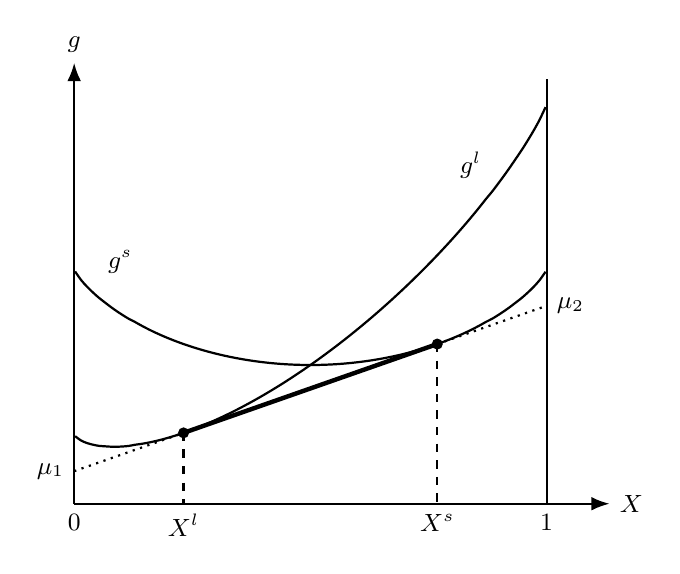
\begin{tikzpicture}[font=\small, >=Latex, line width=0.8pt]
    % axes: X from 0 to 1 (x = 6X), g plotted as 3.5(g+0.85)
    \draw[->] (0,0) -- (6.8,0) node[right] {$X$};
    \draw[->] (0,0) -- (0,5.6) node[above] {$g$};
    \draw (6,0) -- (6,5.4);
    \node[below] at (0,0) {$0$};
    \node[below] at (6,0) {$1$};
    % solid: ideal solution, mu_i^s = 0, k_BT = 0.5
    \draw[domain=0.002:0.998, smooth, samples=80, variable=\t]
        plot ({6*\t},{3.5*(0.85+0.5*(\t*ln(\t)+(1-\t)*ln(1-\t)))});
    % liquid: mu_1^l = -0.6, mu_2^l = +0.6
    \draw[domain=0.002:0.998, smooth, samples=80, variable=\t]
        plot ({6*\t},{3.5*(0.85-0.6*(1-\t)+0.6*\t+0.5*(\t*ln(\t)+(1-\t)*ln(1-\t)))});
    % common tangent: slope 0.6, intercepts mu_1 = -0.732, mu_2 = -0.132
    \draw[dotted] (0,0.414) -- (1.389,0.900);
    \draw[line width=1.6pt] (1.389,0.900) -- (4.611,2.028);
    \draw[dotted] (4.611,2.028) -- (6,2.514);
    \fill (1.389,0.900) circle (2pt);
    \fill (4.611,2.028) circle (2pt);
    \draw[dashed] (1.389,0.900) -- (1.389,0) node[below] {$X^l$};
    \draw[dashed] (4.611,2.028) -- (4.611,0) node[below] {$X^s$};
    % intercepts
    \node[left] at (0,0.414) {$\mu_1$};
    \node[right] at (6,2.514) {$\mu_2$};
    % labels
    \node[left] at (5.3,4.3) {$g^l$};
    \node[above right] at (0.3,2.8) {$g^s$};
\end{tikzpicture}
\end{document}
